
        \documentclass[12p]{article}
        \usepackage[margin=1in, left=1.5in, includefoot]{geometry}
        \usepackage{longtable, tabu}
        \usepackage[table, dvipsnames]{xcolor}
        \usepackage{array,booktabs}
        \usepackage{color}
        \usepackage{indentfirst}
        \usepackage{graphicx}
        \usepackage{float}
        \usepackage[utf8]{inputenc}
        \usepackage{listings}
        \usepackage{url}
        \usepackage{multirow}
        \usepackage{seqsplit}
        
        \definecolor{ferrarired}{rgb}{1.0, 0.11, 0.0}
        \definecolor{orange(colorwheel)}{rgb}{1.0, 0.5, 0.0}
        \definecolor{deepskyblue}{rgb}{0.0, 0.75, 1.0}
        \definecolor{grannysmithapple}{rgb}{0.66, 0.89, 0.63}
        \definecolor{gray(x11gray)}{rgb}{0.75, 0.75, 0.75}
        \definecolor{amber}{rgb}{1.0, 0.75, 0.0}
        
        \newcommand{\icon}[1]{\includegraphics[height=12pt]{#1}}
        \newcommand{\hash}[1]{{\ttfamily\seqsplit{#1}}}

        \setlength{\arrayrulewidth}{0.3mm}
\setlength{\tabcolsep}{18pt}
\renewcommand{\arraystretch}{1.5}
\setlength{\parindent}{1em}
\begin{document}
\begin{titlepage}
\begin{center}
\line(1,0){320}\\
[0.25in]
\huge{\bfseries Android Analysis Report}
\line(1,0){320}\\
[0.5in]
\begin{figure}[H]
	\centering
	
\includegraphics[scale=0.5]{/home/miki/Documents/GITHUB/AndroidPermissions/python/vulns/report_icons/logo.png}
\end{figure}
\textsl{\LARGE Demo app}\\
\textsf{\LARGE edu.ksu.cs.benign}\\
[2.5in]
\end{center}
\begin{flushright}
\textbf{\large Date 2018-06-15}
\end{flushright}
\end{titlepage}
\tableofcontents
\thispagestyle{empty}
\cleardoublepage
\setcounter{page}{1}
\section{PERMISSIONS}
	\begin{longtable}{p{3cm} p{10cm} }
	\rowcolor{grannysmithapple!70} Type & List \\
\hline
Dangerous &  ACCESS\_COARSE\_LOCATION \\ 
 &  ACCESS\_FINE\_LOCATION \\ 
\hline
\hline
Underprivileged &  ACCESS\_COARSE\_LOCATION \\ 
 &  ACCESS\_FINE\_LOCATION \\ 
\hline
\hline
	\end{longtable}
\cleardoublepage
\newpage
\section{FINDINGS SUMMARY}\label{sec:summary}
\begin{figure}[H]
\centering
	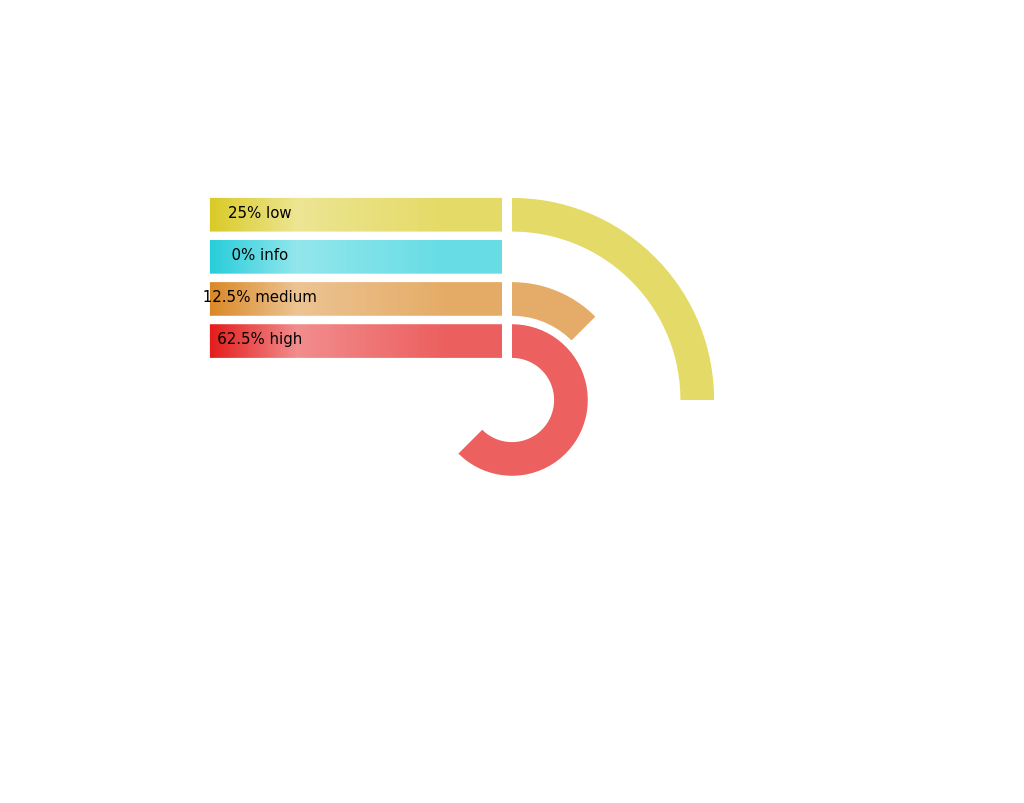
\includegraphics[scale=0.5]{/home/miki/Documents/GITHUB/AndroidPermissions/apks/crypto/ConstantKey_ForgeryAttack_Lean_secure/report/pie_chart.png}
\end{figure}
	\begin{longtable}{p{0.5cm} p{10cm} p{1.5cm}}
	\rowcolor{grannysmithapple!70} Index & Title & Impact \\
	A1&Electronic Codebook \newline (ECB) used for encryption& \color{ferrarired}\textbf{High} \\
\hline\\	\end{longtable}
\cleardoublepage
\newpage
\section{DETAILED FINDINGS}
\subsection{A1: Electronic Codebook (ECB) used for encryption}
\subsubsection*{\protect\icon{/home/miki/Documents/GITHUB/AndroidPermissions/python/vulns/report_icons/basic_sheet.png} Description}

            Using the same encryption key, in ECB mode data blocks are enciphered individually 
            from each other and cause identical message blocks to be transformed to identical ciphertext 
            blocks. The independency of encrypted blocks also implies that the malicious substitution of a 
            block has no impact on adjacent blocks. As a consequence, data patterns are not well hidden and 
            message confidentiality may be compromised.
            
            On Android, the Cipher API provides access to implementations of cryptographic schemes
            for the encryption and decryption of arbitrary data. To request an instance of a particular cipher,
            an application has to invoke the method getInstance, passing a suitable transformation string as
            parameter. Typically, this value is composed of the desired algorithm name, a mode of operation,
            and the padding scheme to apply. For example, to request an object instance that provides AES in
            ECB mode with PKCS5 padding, the transformation AES/ECB/PKCS5Padding has to be specified.
            
            While it is indispensable to declare the algorithm to use, explicitly setting the mode and
            padding may be omitted. To fill the gap, the underlying Cryptographic Service Provider (CSP)
            relies on predefined values that do not necessarily reflect the recommended practice. Precisely, if
            the transformation indicates no operation mode, ECB mode is put in place. Moreover, the initially
            described problem with ECB is not limited to a specific cipher, such as AES but affects all symmetric
            block ciphers. Stream ciphers and asymmetric cryptosystems are not concerned since they
            do not involve an operation mode to repeatedly encipher blocks of contiguous data.
        
\subsubsection*{\protect\icon{/home/miki/Documents/GITHUB/AndroidPermissions/python/vulns/report_icons/basic_magnifier.png} Evidence}
\path{/home/miki/Documents/GITHUB/AndroidPermissions/apks/crypto/ConstantKey_ForgeryAttack_Lean_secure/app/smali/edu/ksu/cs/benign/ResetPasswordActivity$1.smali}

\subsubsection*{\protect\icon{/home/miki/Documents/GITHUB/AndroidPermissions/python/vulns/report_icons/basic_todo.png} Recommendation}
It is recommended not to use ECB for encryption. Use an asymmetric encryption algorithm instead
\cleardoublepage
\newpage
\section{VISUALIZATIONS}
\subsection{Chord Diagram - Class Relations}
\begin{figure}[H]
	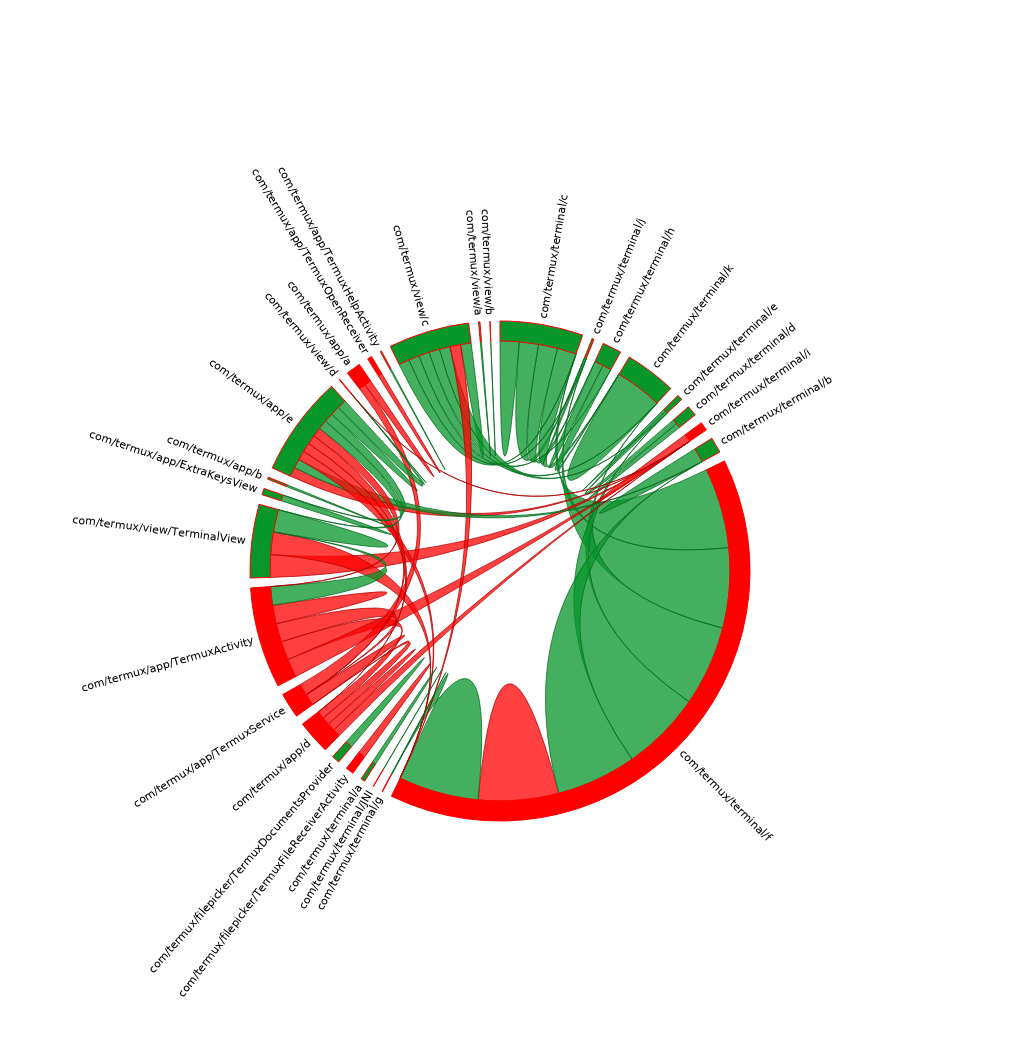
\includegraphics[scale=0.45]{/home/miki/Documents/GITHUB/AndroidPermissions/apks/crypto/ConstantKey_ForgeryAttack_Lean_secure/report/chord_diagram.png}\end{figure}\subsection{Hot Spot - System Overview}
\begin{figure}[H]
\centering
	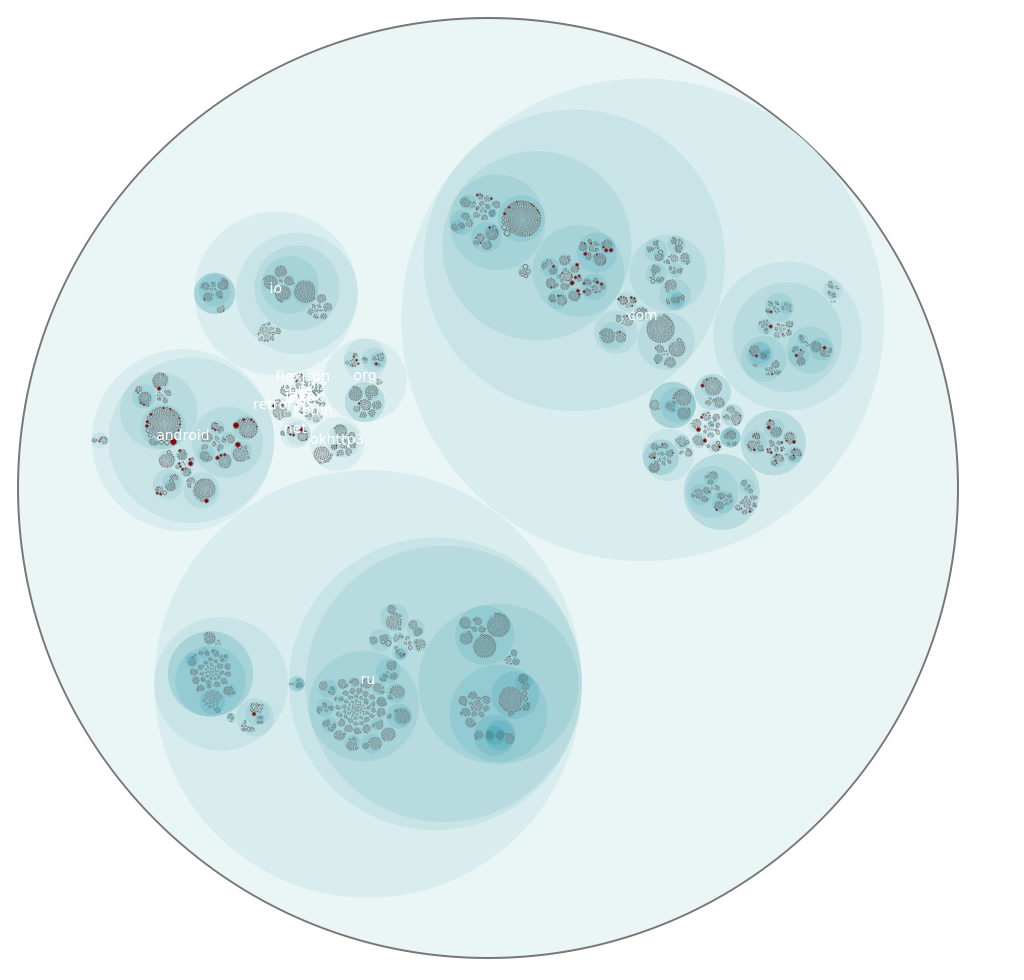
\includegraphics[scale=0.5]{/home/miki/Documents/GITHUB/AndroidPermissions/apks/crypto/ConstantKey_ForgeryAttack_Lean_secure/report/hotspot.png}\end{figure}\begin{longtable}{p{0.3cm} p{12cm}}
\rowcolor{orange} Index & Class \\
1 & \path{/home/miki/Documents/GITHUB/AndroidPermissions/apks/crypto/ConstantKey_ForgeryAttack_Lean_secure/app/smali/edu/ksu/cs/benign/ResetPasswordActivity$1.smali} \\
2 & \path{/home/miki/Documents/GITHUB/AndroidPermissions/apks/crypto/ConstantKey_ForgeryAttack_Lean_secure/app/smali/android/arch/lifecycle/SingleGeneratedAdapterObserver.smali} \\
3 & \path{/home/miki/Documents/GITHUB/AndroidPermissions/apks/crypto/ConstantKey_ForgeryAttack_Lean_secure/app/smali/android/arch/lifecycle/Lifecycle.smali} \\
4 & \path{/home/miki/Documents/GITHUB/AndroidPermissions/apks/crypto/ConstantKey_ForgeryAttack_Lean_secure/app/smali/android/arch/lifecycle/CompositeGeneratedAdaptersObserver.smali} \\
5 & \path{/home/miki/Documents/GITHUB/AndroidPermissions/apks/crypto/ConstantKey_ForgeryAttack_Lean_secure/app/smali/android/arch/lifecycle/LifecycleOwner.smali} \\
6 & \path{/home/miki/Documents/GITHUB/AndroidPermissions/apks/crypto/ConstantKey_ForgeryAttack_Lean_secure/app/smali/android/arch/lifecycle/FullLifecycleObserver.smali} \\
7 & \path{/home/miki/Documents/GITHUB/AndroidPermissions/apks/crypto/ConstantKey_ForgeryAttack_Lean_secure/app/smali/android/arch/lifecycle/LifecycleRegistryOwner.smali} \\
8 & \path{/home/miki/Documents/GITHUB/AndroidPermissions/apks/crypto/ConstantKey_ForgeryAttack_Lean_secure/app/smali/android/arch/lifecycle/AndroidViewModel.smali} \\
9 & \path{/home/miki/Documents/GITHUB/AndroidPermissions/apks/crypto/ConstantKey_ForgeryAttack_Lean_secure/app/smali/android/arch/lifecycle/Lifecycle$Event.smali} \\
10 & \path{/home/miki/Documents/GITHUB/AndroidPermissions/apks/crypto/ConstantKey_ForgeryAttack_Lean_secure/app/smali/android/arch/lifecycle/LifecycleObserver.smali} \\
	\end{longtable}
\end{document}
